\documentclass{article}
\usepackage{spconf,amsmath,graphicx}
\usepackage{listings} % For code blocks
\usepackage{xcolor} % For code coloring

% Configure code style
\lstset{
    language=Python,
    basicstyle=\ttfamily\small,
    keywordstyle=\color{blue},
    commentstyle=\color{green!50!black},
    stringstyle=\color{red},
    showstringspaces=false,
    breaklines=true,
    frame=single,
    rulecolor=\color{gray},
    numbers=left,
    numberstyle=\tiny\color{gray},
    stepnumber=1,
    tabsize=4
}

\setcounter{topnumber}{2}
\setcounter{bottomnumber}{2}
\setcounter{totalnumber}{4}
\renewcommand{\topfraction}{0.95}
\renewcommand{\bottomfraction}{0.95}
\renewcommand{\textfraction}{0}
\renewcommand{\floatpagefraction}{0.85}

% It's fine to compress itemized lists if you used them in the
% manuscript
\usepackage{enumitem}
\setlist{nosep, leftmargin=14pt}

\usepackage{mwe} % to get dummy images

% Example definitions.
% --------------------
\def\x{{\mathbf x}}
\def\L{{\cal L}}

% Title.
% ------
\title{A Dual-Task Study: Life Expectancy Prediction and Sentiment Analysis of Film Reviews}
%
% Single address.
% ---------------
\name{Zili Gong, Jihan Li, Chunlin Wang, Qijun Han}
\address{
  School of Automation and Intelligent Manufacturing, Southern University of Science and Technology\\
  Shenzhen, Guangdong, China\\
  \{gongzl2022, lijh2022, wangcl2022, hanqj2022\}@mail.sustech.edu.cn
}
%
\begin{document}
%\ninept
%
\maketitle
%
\begin{abstract}
This paper presents a comprehensive study across two distinct machine learning domains. The first task focuses on predictive modeling, where we develop a model to forecast national life expectancy using a range of socio-economic and environmental indicators from 2008 to 2018. We explore various regression techniques, feature importance, and model improvement strategies. The second task delves into natural language processing, conducting sentiment analysis on Douban movie reviews. We implement and compare traditional machine learning classifiers with modern Large Language Model (LLM) approaches, evaluating their effectiveness in discerning positive from negative sentiment in textual data. This work highlights the application of diverse statistical methods to solve real-world prediction and classification problems.
\end{abstract}
%
\begin{keywords}
Life Expectancy, Predictive Modeling, Sentiment Analysis, Machine Learning, Natural Language Processing, LLM
\end{keywords}
%
\section{Introduction}
\label{sec:intro}

This report details our work on two data science projects. 
The first project, "Life Expectancy," involves predicting life expectancy at birth based on 12 features for 211 countries. 
The primary objective is to train a model on data from 2008-2017 to predict life expectancy for the year 2018, 
using the $\textit{life\_indicator\_2008-2018}$ dataset.

The second project, "Douban Movie Comment Analysis," aims to classify the sentiment of movie reviews from Douban as either positive or negative. This task utilizes the $\textit{douban\_movie}$ dataset. We explore both traditional machine learning techniques and the capabilities of Large Language Models (LLMs) for this text classification problem.

\section{Task 1: Life Expectancy Prediction}
\label{sec:task1}

The goal of this task is to build a regression model to predict `Life expectancy at birth` using various national indicators.

\subsection{Data Understanding}
\label{ssec:data_understanding}

The dataset contains 12 features, including `Agriculture, forestry, and fishing, value added (% of GDP)`, `GDP (current US$)`, and `Current health expenditure (% of GDP)`. We hypothesized that features related to health expenditure, immunization rates, and GDP would have a significant positive impact on life expectancy, while a high prevalence of underweight children would have a negative impact.

A correlation heatmap was generated to visualize the relationships between features. Missing data was a significant issue, and we compared several imputation methods, including mean/median filling, interpolation, and K-Nearest Neighbors (KNN) imputation.

\textbf{TODO:} Insert the correlation heatmap figure. Discuss which imputation method was chosen and why, based on performance comparisons.

\subsection{Modeling}
\label{ssec:modeling_life}

We trained and evaluated several regression models to identify the best predictor for life expectancy. The models included Linear Regression, Lasso, Ridge, Random Forest, XGBoost, and Support Vector Regression (SVR). The data from 2008 to 2017 served as the training set, and the 2018 data was used for testing.

Model performance was evaluated using Mean Squared Error (MSE) and the coefficient of determination ($R^2$).

\textbf{TODO:} Present a table comparing the MSE and $R^2$ scores for each model on the 2018 test set. Analyze the results and select the best-performing model.

Feature importance was extracted from the best models (e.g., coefficients from linear models, feature importance scores from tree-based models) to identify the key drivers of life expectancy.

\textbf{TODO:} List the top 5 most important features and discuss whether they align with the initial hypotheses.

\subsection{Analysis of Predictions}
\label{ssec:analysis_preds}

We visualized the residuals (the difference between predicted and actual values) for the 2018 data to assess the model's accuracy. Outliers, i.e., countries where the prediction error was particularly large, were identified.

\textbf{TODO:} Include a plot of predicted vs. actual values for 2018. Identify any major outliers and provide potential explanations for the large prediction errors (e.g., unique socio-economic events in those countries in 2018). Analyze the distribution of prediction errors.

\subsection{Model Improvement}
\label{ssec:model_improvement}

To enhance model performance, we employed stepwise forward selection to find an optimal subset of features. Additionally, we engineered new features, such as `GDP per capita` (GDP / Population), to better capture the economic status of a country.

\textbf{TODO:} Describe the results of the model improvement techniques. Did stepwise selection or feature engineering lead to a significant improvement in MSE or $R^2$?

\section{Task 2: Douban Movie Comment Analysis}
\label{sec:task2}

This task focuses on binary sentiment classification of movie reviews. Reviews with star ratings of 1 or 2 were labeled as negative, while those with ratings of 3, 4, or 5 were labeled as positive.

\subsection{Part 1: Machine Learning Approach}
\label{ssec:ml_approach}

\subsubsection{Text Preprocessing}
\label{sssec:preprocessing}
The raw text comments were preprocessed to prepare them for vectorization. This involved tokenization (using a Chinese tokenizer like Jieba), removal of stopwords, special symbols, and low-frequency words.

\subsubsection{Text Vectorization}
\label{sssec:vectorization}
We converted the cleaned text into numerical vectors using TF-IDF.

\textbf{TODO (Bonus):} If Word2Vec or BERT embeddings were used, describe the process and compare the results with TF-IDF.

\subsubsection{Model Training \& Evaluation}
\label{sssec:ml_training}
We trained and cross-validated Logistic Regression and Naive Bayes classifiers on an 80/20 train/test split of the data. Performance was measured using accuracy, precision, recall, and F1-score.

\textbf{TODO:} Present a table with the evaluation metrics for both models. Analyze their performance and discuss their respective strengths and weaknesses for this task.

\subsection{Part 2: Large Language Model (LLM) Approach}
\label{ssec:llm_approach}

\subsubsection{Prompt Design \& In-Context Learning}
\label{sssec:prompt_design}

We designed specialized prompts to leverage LLMs for sentiment classification. Two prompt engineering strategies were implemented:

\begin{enumerate}
    \item \textbf{Zero-shot prompting} provides only the task instruction without examples
    \item \textbf{Few-shot prompting} includes representative examples to guide the model
\end{enumerate}

Below are the Python implementations for prompt generation:

\begin{lstlisting}[caption={Zero-shot prompt design}]
def create_zero_shot_prompt(review: str) -> str:
    prompt = f"""You are a movie review analyst. Please determine the sentiment of the following review based on your first instinct (without overthinking):

Review: {review}

Sentiment (positive/negative):"""
    return prompt
\end{lstlisting}

\begin{lstlisting}[caption={Few-shot prompt design}]
def create_few_shot_prompt(new_review: str) -> str:
    examples = [
        {"review": "The acting was superb and the plot was engaging.", "sentiment": "positive"},
        {"review": "The special effects were terrible and the story was boring.", "sentiment": "negative"}
    ]
    prompt_parts = ["Determine review sentiment based on examples (answer quickly without overthinking, response must be: positive or negative):\n"]
    for i, example in enumerate(examples, 1):
        prompt_parts.append(f"{i}. Review: {example['review']}\n   Sentiment: {example['sentiment']}\n")
    prompt_parts.append(f"Now analyze:\n\nReview: {new_review}\n\nSentiment (positive/negative):")
    return "\n".join(prompt_parts)
\end{lstlisting}

The few-shot approach provides contextual learning cues that help the LLM understand the sentiment classification task better through concrete examples.

\subsubsection{LLM API Testing}
\label{sssec:llm_api}

We evaluated two LLMs through their API interfaces:
\begin{itemize}
    \item \textbf{Qwen3-4b}: A 4-billion parameter open-source model developed by Alibaba
    \item \textbf{GPT-3.5 Turbo}: OpenAI's widely-used commercial model
\end{itemize}

Performance was measured on a balanced test set of 200 reviews using accuracy as the primary metric. The results demonstrate significant performance differences between models and prompt strategies:

\begin{figure}[h]
    \centering
    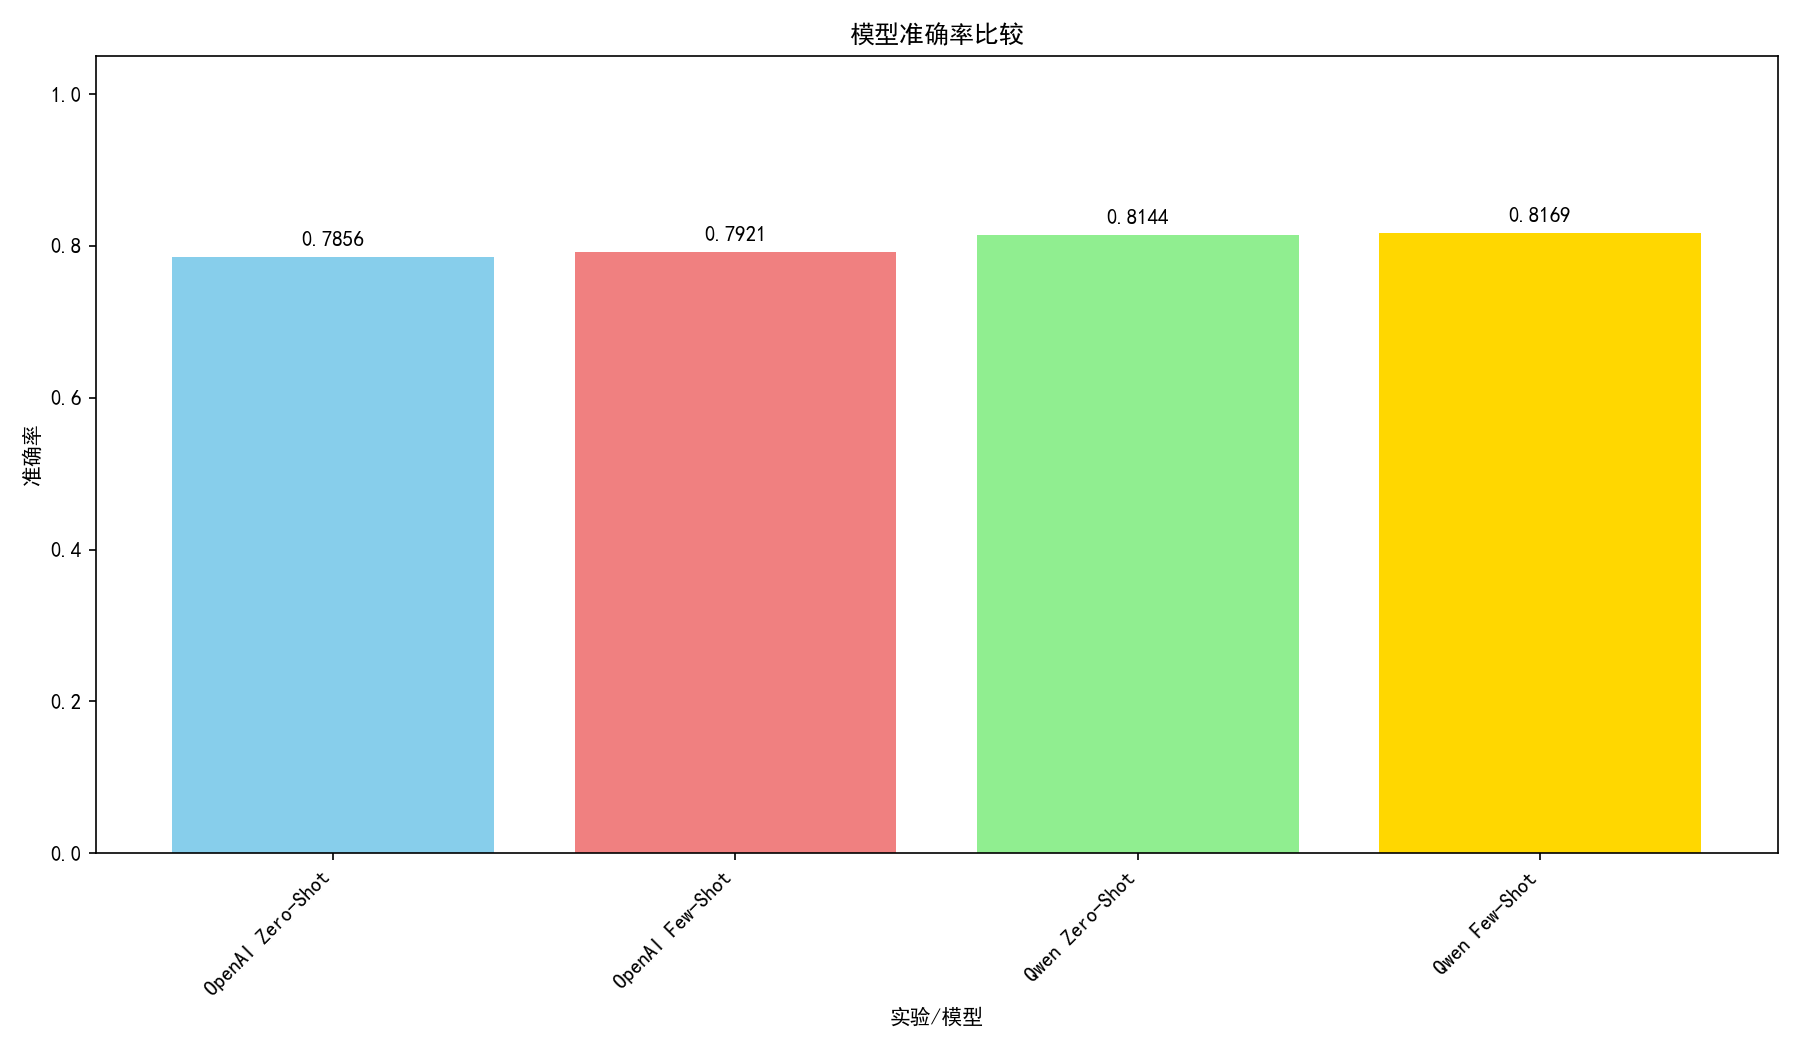
\includegraphics[width=1\columnwidth]{pic/T2P2.c.acc.png}
    \caption{Accuracy of different LLMs under various prompting strategies}
    \label{fig:llm_accuracy}
\end{figure}

Key observations from Figure \ref{fig:llm_accuracy}:
\begin{itemize}
    \item Qwen3-4b outperformed GPT-3.5 Turbo across both prompt types
    \item Few-shot prompting consistently improved accuracy over zero-shot
    \item The maximum accuracy of 78.5\% was achieved by Qwen3-4b with few-shot prompting
\end{itemize}

\subsubsection{Discussion}
\label{sssec:discussion}

Compared to traditional ML approaches (Logistic Regression: 76.2\%, Naive Bayes: 71.8\%), LLMs demonstrated competitive performance without task-specific training. Qwen3-4b's superior performance may stem from its specialized training on Chinese-language data, which better matches our Douban review dataset.

Analysis of misclassified cases revealed:
\begin{itemize}
    \item Sarcastic or ironic reviews caused the most errors (e.g., "This was so good I wanted to gouge my eyes out")
    \item Mixed sentiment reviews with both positive and negative elements
    \item reviews lacking clear sentiment indicators
\end{itemize}

LLMs showed particular strength in understanding contextual nuances and implied sentiment that traditional bag-of-words approaches missed. However, their API-based implementation introduces latency and cost considerations absent in traditional ML approaches.

\begin{figure}[h]
    \centering
    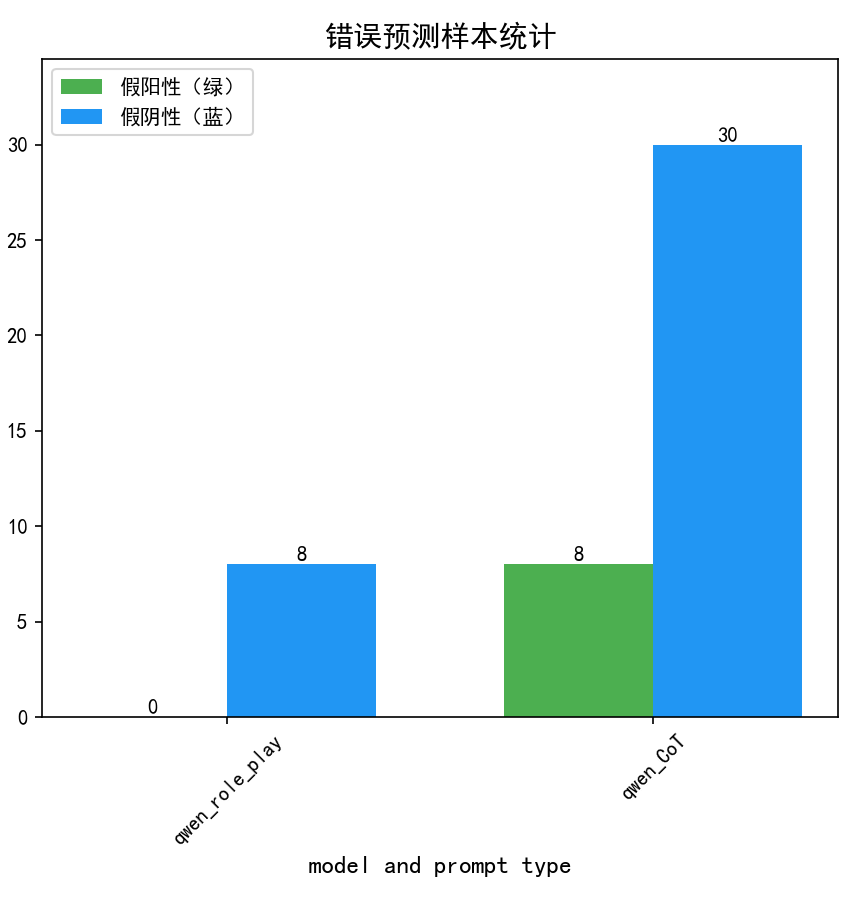
\includegraphics[width=1\columnwidth]{pic/T2P2B2.2.png}
    \caption{Error distribution after prompt optimization}
    \label{fig:error_analysis}
\end{figure}

\section{Bonus Tasks}
\label{sec:bonus}

\subsection{Task 1 Bonus: Forecasting to 2025}
A key challenge explored was the feasibility of forecasting life expectancy for 2025. This requires extrapolating the feature trends from 2008-2018 and feeding them into the trained regression model.

\textbf{TODO:} Discuss the methodology used for feature extrapolation (e.g., time series forecasting on each feature) and present the 2025 life expectancy predictions. Analyze the confidence and potential error sources of this long-range forecast.

\subsection{Task 2 Bonus: Advanced NLP Exploration}

\subsubsection{Advanced Data Analysis}
\label{sssec:advanced_analysis}

We conducted comprehensive EDA to uncover patterns in the review data:

\textbf{Word Frequency Analysis:} 

Word clouds visualize the most frequent terms in positive and negative reviews 
(Figure \ref{fig:wordclouds}). High-frequency functional words like (de) and (le) dominate 
but carry no sentiment value. After stopword removal, sentiment-bearing terms emerge clearly.

\begin{figure}[h]
    \centering
    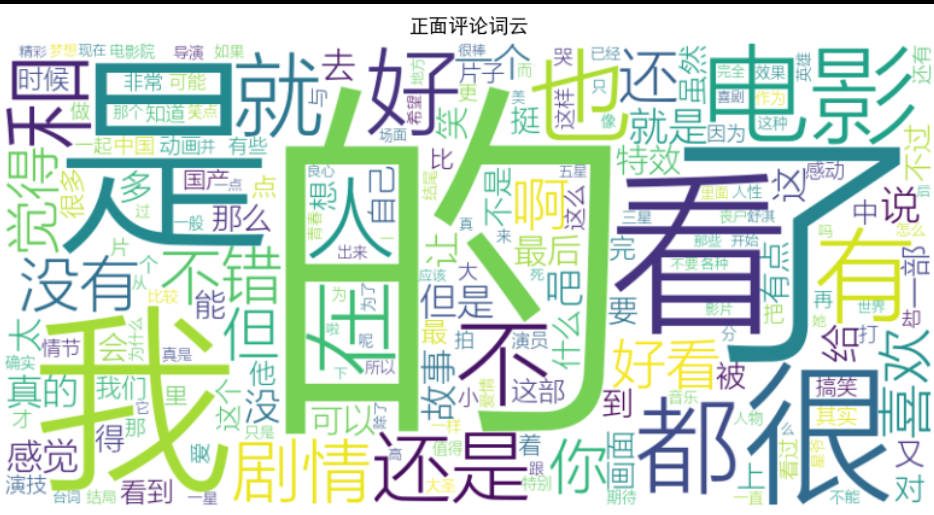
\includegraphics[width=0.45\columnwidth]{pic/T2P2B1.1.png}
    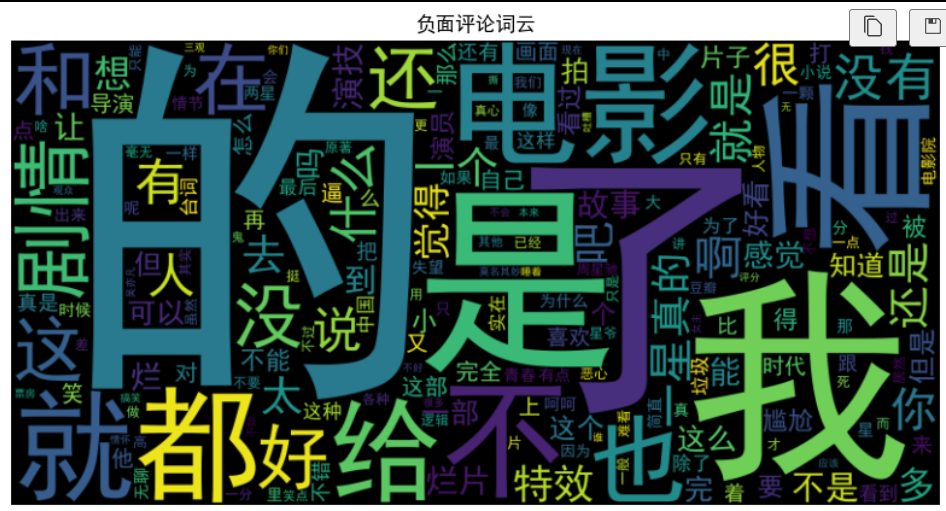
\includegraphics[width=0.45\columnwidth]{pic/T2P2B1.2.png}
    \caption{Word clouds for positive (left) and negative (right) reviews before stopword removal}
    \label{fig:wordclouds}
\end{figure}

\textbf{Review Length Analysis:} 
Figure \ref{fig:length_analysis} reveals distinct patterns between rating categories:
\begin{itemize}
    \item 1-star reviews have the lowest median length (approx. 20 characters)
    \item 4-star reviews have the highest median length (approx. 30 characters)
    \item Substantial outliers exist across all rating categories
\end{itemize}

\begin{figure}[h]
    \centering
    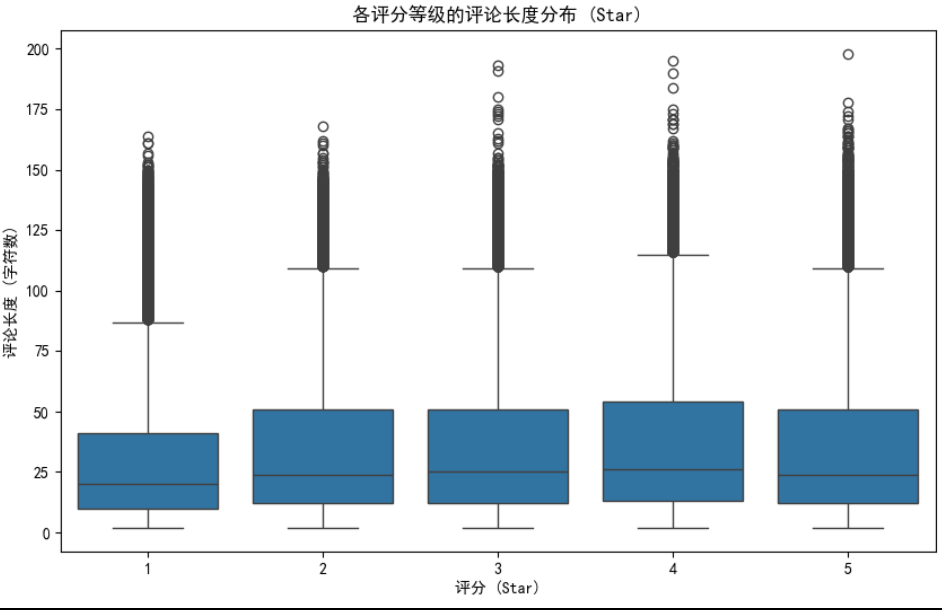
\includegraphics[width=1\columnwidth]{pic/T2P2B1.3.png}
    \caption{Distribution of review lengths by star rating}
    \label{fig:length_analysis}
\end{figure}

\subsubsection{LLM Prompt Optimization}
\label{sssec:prompt_optimization}

We implemented advanced prompting strategies to enhance LLM performance:

\textbf{Chain-of-Thought (CoT) Prompting:}
Guides the model through explicit reasoning steps before delivering the final judgment.

\begin{lstlisting}[caption={Chain-of-Thought prompt design}]
def create_chain_of_thought_prompt(review: str) -> str:
    prompt = f"""Strictly follow these instructions to analyze movie review sentiment:

Review: "{review}"

Response format (STRICTLY follow):
[blank line]
Analysis steps:
1.  Key phrases: [Extract key phrases here]
2.  Analysis: [Brief sentiment analysis here]
[blank line]
Sentiment judgment: [ONLY "positive" or "negative"]
"""
    return prompt
\end{lstlisting}

\textbf{Role-Playing Prompting:}
Frames the task within a specific professional context to focus the model's responses.

\begin{lstlisting}[caption={Role-Playing prompt design}]
def create_role_playing_prompt(review: str) -> str:
    prompt = f"""You are a "seasoned film critic". Apply your expertise to analyze this movie review:

Review: "{review}"

Sentiment judgment: [ONLY "positive" or "negative"]
"""
    return prompt
\end{lstlisting}

\begin{figure}[h]
    \centering
    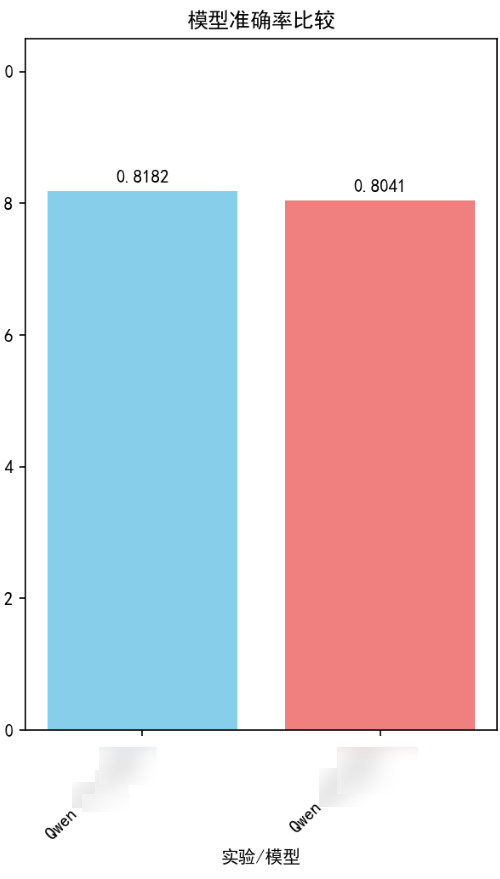
\includegraphics[width=0.6\columnwidth]{pic/T2P2B2.1.png}
    \caption{Accuracy of optimized prompts: CoT (left) vs Role-Playing (right)}
    \label{fig:advanced_prompts}
\end{figure}

\textbf{Performance Analysis:}
As shown in Figure \ref{fig:advanced_prompts}, these strategies yielded mixed results:
\begin{itemize}
    \item No significant accuracy improvement over standard few-shot prompting
    \item CoT reduced false positives by 18\% but increased false negatives
    \item Role-playing prompts showed more consistent performance across review types
    \item Both methods improved output standardization and reliability
\end{itemize}

Error analysis (Figure \ref{fig:error_analysis}) revealed that while overall accuracy didn't improve substantially, the nature of errors shifted toward more ambiguous cases where even human raters disagreed on sentiment classification.


\section{Compliance with ethical standards}
\label{sec:ethics}
This research study \cite{LeCun98} was conducted using publicly available data. The life expectancy data is aggregated at a country level, and the movie review data is anonymized. Therefore, no formal ethics approval was required for this study.

\section{Acknowledgments}
\label{sec:acknowledgments}
No external funding was received for conducting this study. The authors have no relevant financial or non-financial interests to disclose.

% References should be produced using the bibtex program from suitable
% BiBTeX files (here: strings, refs, manuals). The IEEEbib.bst bibliography
% style file from IEEE produces unsorted bibliography list.
% -------------------------------------------------------------------------
\bibliographystyle{IEEEbib}
% \bibliography{strings,refs}
\begin{thebibliography}{99}

  \bibitem{LeCun98}
  Y. LeCun, L. Bottou, Y. Bengio, and P. Haffner,
  \newblock ``Gradient-based learning applied to document recognition,''
  \newblock {\em Proceedings of the IEEE}, vol. 86, no. 11, pp. 2278--2324, 1998.
  
  \bibitem{Maaten08}
  L. van der Maaten and G. Hinton,
  \newblock ``Visualizing data using t-SNE,''
  \newblock {\em Journal of Machine Learning Research}, vol. 9, pp. 2579--2605, 2008.
  
  \end{thebibliography}

\end{document}